\section[Обзор технологии WebRTC]{%
  ОБЗОР ТЕХНОЛОГИИ WEBRTC
}
\label{sec:webrtc}

\subsection{Общая характеристика}
\label{ssec:webrtc_overview}

\textbf{WebRTC} (web real-time communications) --- стандарт, 
который позволяет передавать аудио и видео данные от браузера к браузеру
в режиме реального времени без установки дополнительных плагинов.

Преимущества технологии WebRTC:
\begin{itemize}
\item экономия времени пользователей на установку и поддержку расширений или плагинов,
  а также легкое подключение к видеоконференции;
\item обеспечение более высокого уровня безопасности, чем большинство современных систем
  телефонной связи;
\item WebRTC --- проект с открытым кодом;
\end{itemize}

WebRTC является серьезным конкурентом для технологии Flash,
которая ранее использовалась для передачи потоков информации в режиме реального времени,
но требовала установки дополнительных расширений для операционных систем и браузеров.

Использование WebRTC с точки зрения пользователя (клиента) в упрощенном виде 
представляет собой следующую последовательность действий:
\begin{enumerate}
\item Пользователь открывает в веб-браузере страницу, содержащую JavaScript,
  который обрабатывает данные библиотеки WebRTC.
\item Вверху страницы появляется сервисная строка, где можно разрешить или
  запретить передачу медиа-трафика с веб-камеры и микрофона. 
  Чтобы начать вещать аудио и видео, пользователь должен разрешить передачу медиа-трафика.
\item JavaScript получает от библиотеки WebRTC основную сетевую информацию 
  (IP-адреса и порты), для дальнейшего обмена информацией между другими WebRTC клиентами
  (пирами), даже если используется NAT и firewall.
\item При появлении пиров, начинается обмен информацией об аудио и видео кодеках.
  Начинается передача потоковых данных между WebRTC клиентами.
\end{enumerate}

Для обмена данными между двумя участниками видеосервер не требуется,
но если нужно объединить в одной конференции несколько участников, 
включая другие каналы медиа-трафика (например, видеопоток с IP-камер) сервер необходим.

Видеосервер получает медиа-трафик с различных источников, 
преобразовывает его и отправляет пользователям, 
укоторые в качестве терминала используют WebRTC, 
как показано на рисунке~\ref{pic:webrtc_server}.

\begin{figure}[h!]
  \centering
  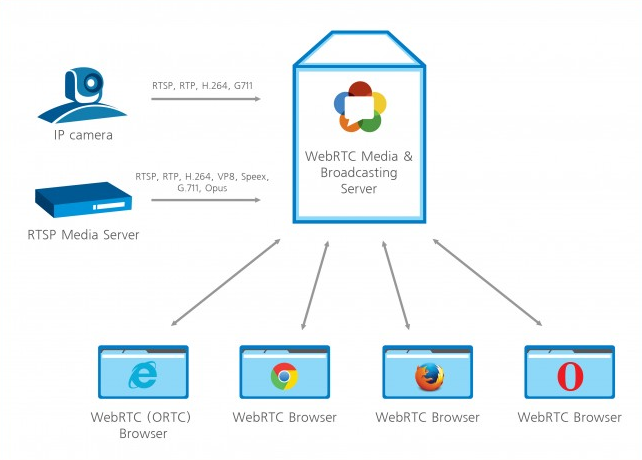
\includegraphics[width=150mm]{pic/webrtc_server.png}
  \caption{Схема работы WebRTC сервера}
  \label{pic:webrtc_server}
\end{figure}

Также WebRTC сервер получает медиа-трафик от WebRTC пиров и передает его
участникам конференции, которые используют приложения для настольных компьютеров 
или мобильных устройств.

\subsection{Программный интерфейс}
\label{ssec:webrtc_api}

Технология WebRTC базируется на трех основных объектах,
предоставляющих программный интерфейс пользователям:

\begin{itemize}
\item \texttt{MediaStream} --- отвечает за принятие приложением аудио и видеосигнала
  от камер или рабочего стола пользователя;
\item \texttt{RTCPeerConnection} --- отвечает за соединение между браузерами для
  обмена полученными медиаданными. 
  Также в <<обязанности>> этого API входит обработка сигнала 
  (очистка его от посторонних шумов, регулировка громкости микрофона) и
  контроль над используемыми аудио и видеокодеками);
\item \texttt{RTCDataChannel} --- обеспечивает двустороннюю передачу произвольных
  данных через установленное соединение.
\end{itemize}

Объект \texttt{MediaStream} состоит из одного или нескольких отдельных треков 
(\texttt{MediaStreamTracks}), которые синхронизированы друг с другом. Содержимое
\texttt{MediaStream} может быть использовано локально или отправлено одному или
нескольким адресатам посредством \texttt{RTCPeerConnection}, 
как показано на рисунке~\ref{pic:webrtc_mediastream}.

\begin{figure}[h!]
  \centering
  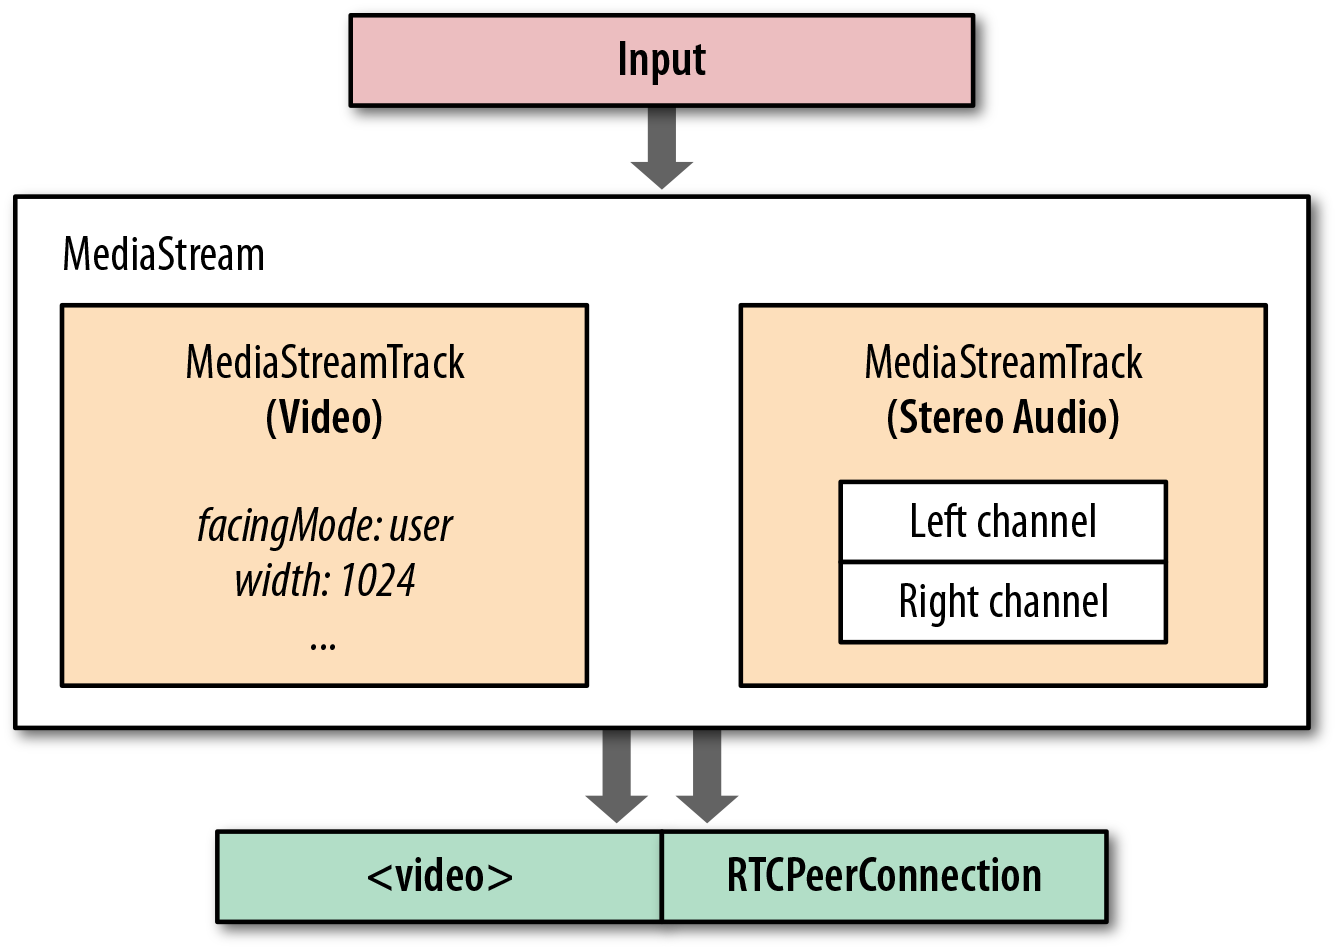
\includegraphics[width=150mm]{pic/webrtc_mediastream.png}
  \caption{Объект \texttt{MediaStream}}
  \label{pic:webrtc_mediastream}
\end{figure}

Объект \texttt{RTCPeerConnection} производит обмен сведениями о параметрах соединения и
медиапотока через некоторый сигнальный канал. Детали работы этого канала не определены
в стандарте для того для того, чтобы сделать его максимально гибким по отношению к
различным потребностям в топологиях соединений и специфике решаемых задач.

В качестве сигнального канала можно использовать следующие решения:
\begin{itemize}
\item SIP (session initiation protocol);
\item Jingle;
\item ISUP (ISDN user part).
\end{itemize}

Объект \texttt{RTCDataChannel} используется для передачи произвольных 
(как бинарных, так и текстовых) пользовательских данных по установленному соединению.

\subsection{Организация передачи данных}
\label{ssec:webrtc_transmission}

Для передачи данных в реальном режиме времени и обеспечения высокого уровня
безопасности используется стек протоколов, представленный на рисунке~\ref{pic:webrtc_stack}.

\begin{figure}[h!]
  \centering
  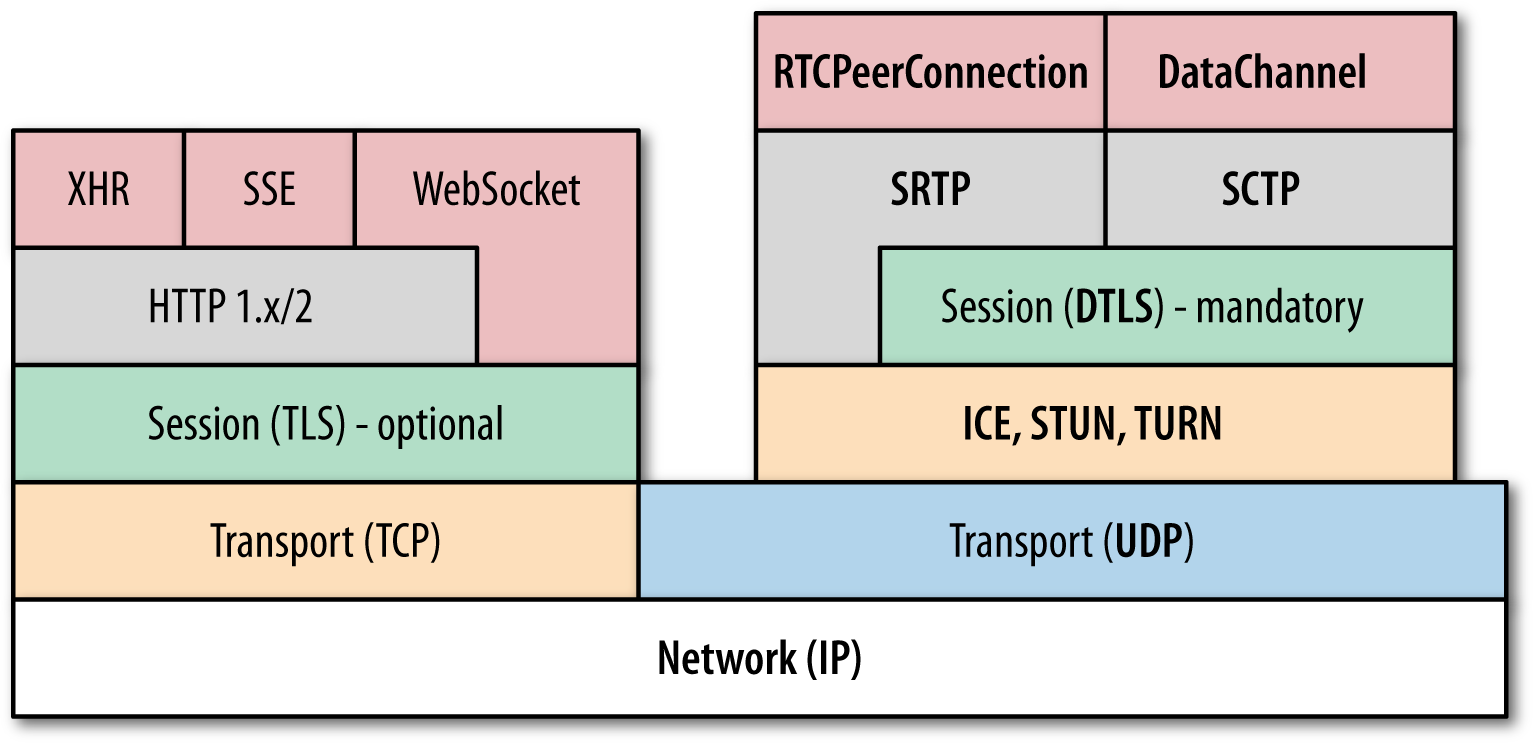
\includegraphics[width=150mm]{pic/webrtc_stack.png}
  \caption{Cтек протоколов, используемых в WebRTC}
  \label{pic:webrtc_stack}
\end{figure}

Столь богатый набор протоколов обусловлен следующими требованиями:
\begin{itemize}
\item задержки передачи данных (jitter) должны быть минимальны;
\item данные должны передаваться в зашифрованном виде.
\end{itemize}

Передача данных в WebRTC производится на базе стека протоколов TCP/IP.
Данные, необходимые для установления и управления соединением, передаются 
по сигнальному каналу на базе протокола TCP c шифрованием TLS.
Медиаданные передаются посредством протокола UDP, не гарантироующего надежность
доставки и сохранность порядка передаваемых дейтаграмм, 
поэтому для передачи данных используются протоколы SRTP и SCTP, поддерживающие 
шифрование. 
Для обмена ключами в процессе установления соединения по ненадежному каналу связи
используется протокол DTLS.

Протокол ICE используется для определения наилучшего варианта конфигурации стека протоколов
передачи мультимедийных данных.
Протоколы STUN и TURN используются для обхода блокировок firewall и
систем трансляций адресов (NAT):
STUN используется для того, чтобы определить, находится ли пользователь за NAT и
определения типа NAT (статический или динамический), а TURN используется для
отправки трафика через TURN-сервер в случае динамического NAT, 
как показано на рисунке~\ref{pic:webrtc_ice}.

\begin{figure}[h!]
  \centering
  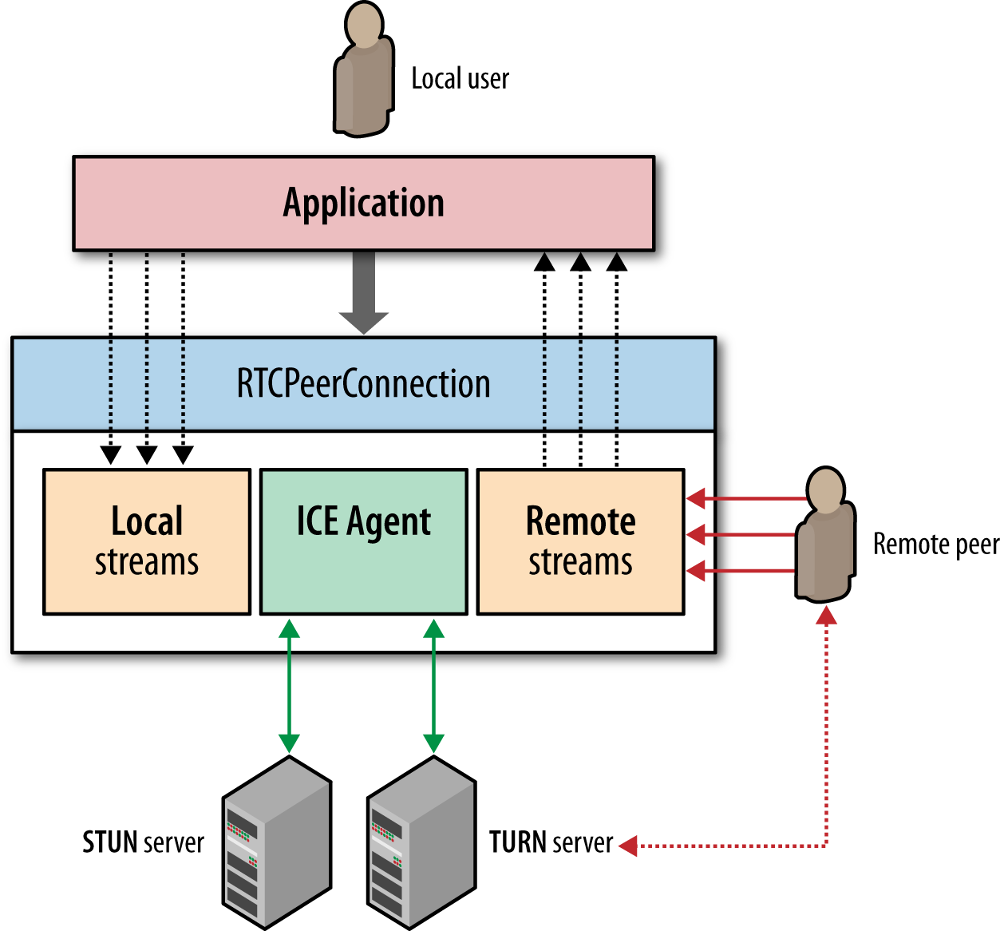
\includegraphics[width=130mm]{pic/webrtc_ice.png}
  \caption{Подсистема управления соединением WebRTC}
  \label{pic:webrtc_ice}
\end{figure}

Процесс установления соединения по сигнальному каналу
представлен на рисунке~\ref{pic:webrtc_establish_conn}.

\begin{figure}[h!]
  \centering
  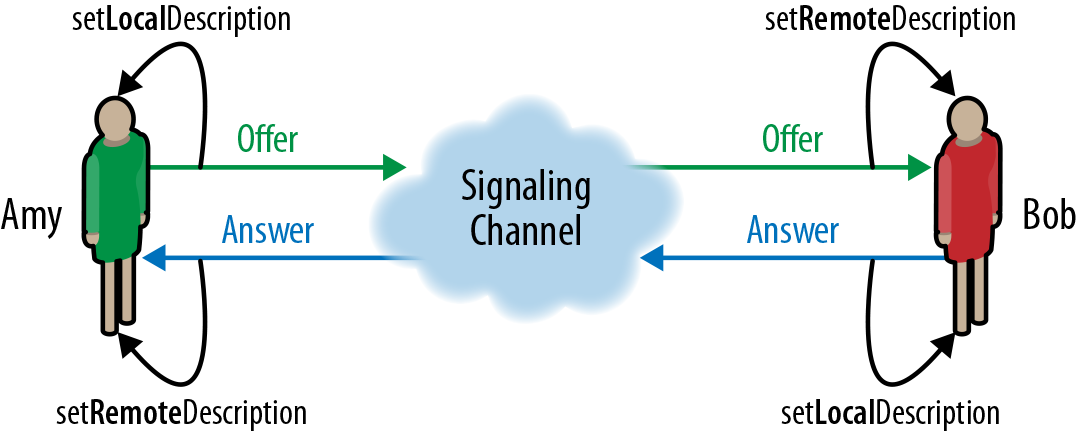
\includegraphics[width=150mm]{pic/webrtc_establish_conn.png}
  \caption{Порядок установления соединения WebRTC}
  \label{pic:webrtc_establish_conn}
\end{figure}

Неформально его описать следующим образом:
\begin{enumerate}
\item Адресант (Amy) регистрирует один или несколько мультимедийных потоков
  с помощью своего локального объекта \texttt{RTCPeerConnection} и устанавливает
  свое локальное описание сессии (local description).
\item Адресант генерирует и посылает предложение установки сессии (session offer)
  адресату (Bob).
\item Адресат получает описание сессии от адресанта,
  устанавливает его в качестве удаленного описания сессии
  (remote session description), регистрирует свои мультимедийные потоки
  в локальном объекте \texttt{RTCPeerConnection}, генерирует ответное сообщение,
  устанавливает его в качестве локального описания сессии и отправляет его адресату.
\item Адресант получает подтверждение от адресата и устанавливает его в качестве 
  собственного удаленного описания сессии.
\end{enumerate}

Схема передачи данных в WebRTC представлена на рисунке~\ref{pic:webrtc_transmission}.

\begin{figure}[h!]
  \centering
  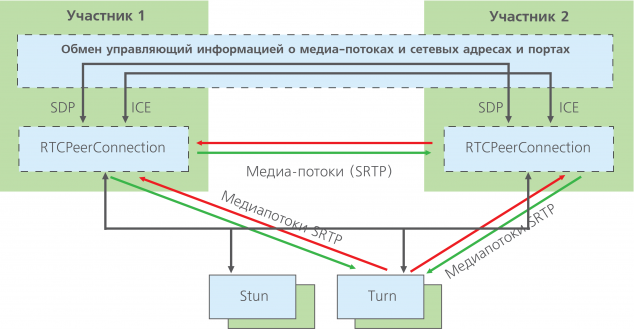
\includegraphics[width=130mm]{pic/webrtc_transmission.png}
  \caption{Потоки передачи данных в WebRTC}
  \label{pic:webrtc_transmission}
\end{figure}

\subsection{Детали реализации}
\label{ssec:webrtc_realization}

На рисунке~\ref{pic:webrtc_architecture} представлена архитектура реализации
стандарта WebRTC. Фиолетовым цветом выделены части, доступные для изменения 
программистам веб-приложений; голубым --- программный интерфейс для разработчиков 
браузеров; зеленым --- внутренние детали реализации библиотеки.

\begin{figure}[h!]
  \centering
  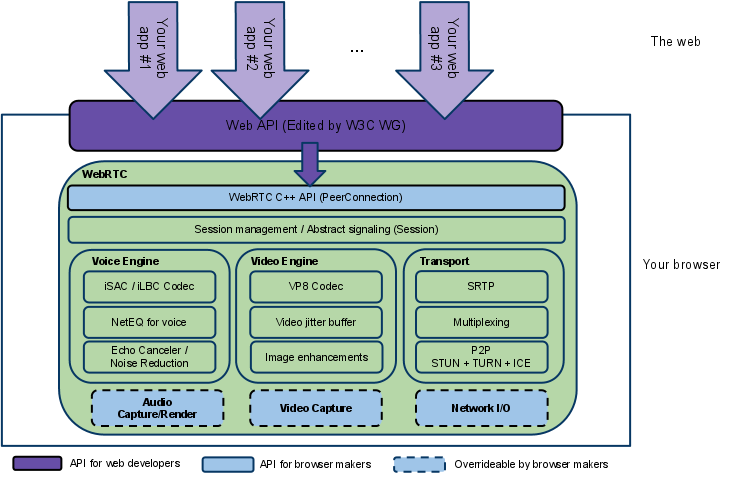
\includegraphics[width=150mm]{pic/webrtc_architecture.png}
  \caption{Архитектура WebRTC}
  \label{pic:webrtc_architecture}
\end{figure}

Кодеки, используемые WebRTC, выполняют следующие задачи:
\begin{itemize}
\item отмена поврежденных пакетов;
\item эхоподавление;
\item адаптация под пропускную способность канала;
\item динамическая буфферизация для нивелирования jittering;
\item автоматическая реулировка громкости;
\item подавление звукового шума и шума видео.
\end{itemize}

Рассмотрим аудиокодеки, используемые в WebRTC.

\textbf{G.711} --- старый голосовой кодек с высоким битрейтом (64 kbps), 
который чаще всего применяется в системах традиционной телефонии. 
Основным достоинством является минимальная вычислительная нагрузка 
из-за использования легких алгоритмов сжатия.
Кодек отличается низким уровнем компрессии голосовых сигналов
и не вносит дополнительной задержки звука во время общения между пользователями.
G.711 поддерживается большим количеством устройств. 
Системы, в которых используется этот кодек, более легкие в применении, 
чем те, которые основаны на других аудиокодеках (G.723, G.726, G.728 и т.д.). 
По качеству G.711 получил оценку 4.2 в тестировании MOS 
(оценка в пределах 4-5 является самой высокой и означает хорошее качество, 
аналогичное качеству передачи голосового трафика в ISDN и даже выше).

\textbf{Opus} --- кодек с низкой задержкой кодирования (от 2{,}5 мс до 60 мс),
поддержкой переменного битрейта и высоким уровнем сжатия, 
что идеально подходит для передачи потокового аудиосигнала в сетях с
переменной пропускной способностью. 
Opus --- гибридное решение, сочетающее в себе лучшие характеристики кодеков SILK
(компрессия голоса, устранение искажений человеческой речи) и CELT
(кодирование аудиоданных). 
Кодек находится в свободном доступе, разработчикам, которые его используют,
не нужно платить отчисления правообладателям. 
По сравнению с другими аудиокодеками, Opus, несомненно, выигрывает по множеству показателей.
Он затмил довольно популярные кодеки с низким битрейтом, такие, как MP3, Vorbis, AAC LC.
Opus восстанавливает более приближенную к оригиналу <<картину>> звука, 
чем AMR-WB и Speex.

Вопросы выбора видеокодека для WebRTC заняли у разработчиков несколько лет,
в итоге решили использовать H.264 и VP8. 
Практически все современные браузеры поддерживают оба кодека.
Серверам видеоконференций для работы с WebRTC достаточно поддеривать только один.

\textbf{VP8} --- свободный видеокодек с открытой лицензией,
отличается высокой скоростью декодирования видеопотока и повышенной устойчивостью к
потере кадров.
Кодек универсален, его легко внедрить в аппаратные платформы, 
поэтому очень часто разработчики систем видеоконференцсвязи используют его 
в своих продуктах.

Платный видеокодек \textbf{H.264} стал известен намного раньше своего собрата.
Это кодек с высокой степенью сжатия видеопотока при сохранении высокого качества видео.
Высокая распространенность этого кодека среди аппаратных систем
видеоконференцсвязи предполагает его использование в стандарте WebRTC.